\subsection{Implementation}
\label{sec:implementation}

The way wollok is implemented is essential to enable us to build a fully customized educational language with a industrial-level toolset.
After many years of experience in the Ozono project and its predecessor, we arrived to the conclussion that
the limitations of a language implemented as an embedded DSL \cite{Mern05a} produce hindrances in the learning process (\cf Sec. \ref{sec:newLanguage}).
Still, giving up the embedded implementation strategy is not conceivable if we have to create all the required tools "from scratch".
Also we require a flexible implementation that allows the language to evolve, enabling and supporting our research activities.

The current implementation of Wollok language is built on top of Xtext\footnote{\url{http://www.eclipse.org/Xtext/}}, 
which is an Eclipse\footnote{\url{https://www.eclipse.org/home/index.php}}-based Language Workbench\cite{fowler2005language}.
By providing a set of tools for language development, the Xtext workbench allows us to get rid of some the necessary effort required to build a language and IDE.
Out from the language grammar, which is defined as an extended BNF, the workbench provides several parts of the infrastructure a language requires: 
a parser, an object-oriented AST representation\footnote{The AST is represented as Java ECore models, which are part of the EMF project \url{http://www.eclipse.org/modeling/emf}}, 
an editor capable of syntax and error highlighting, basic content-assist (\cf \figref{codetemplates.png}) and cross-references search, 
and other tools attached to the IDE, such as structured views of the code (\cf \figref{outline.png}).
Also, it gives us support for implementing more advanced tools such as quick-fixes, refactorings and UI Wizards for creating projects other Wollok entities.
The IDE is integrated into the Eclipse platform, which in turn also helped us integrating with other Eclipse tools, such as the JUnit test runner and a debugger.

\begin{figure}[ht]
    \centering
	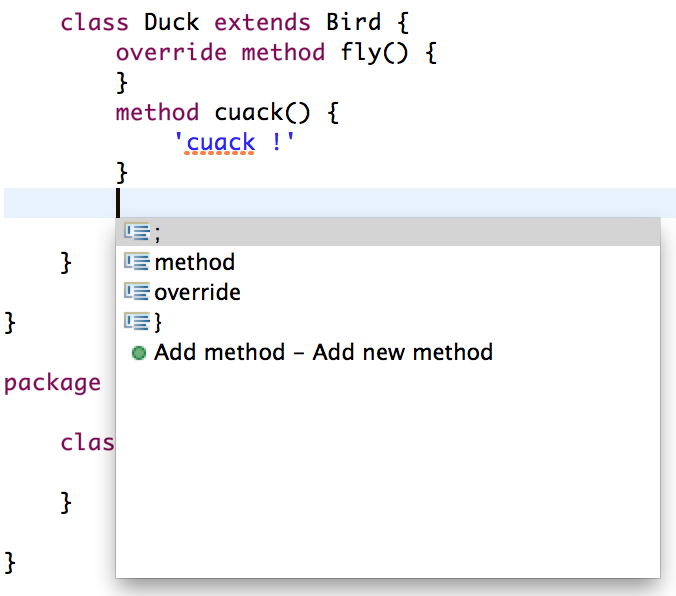
\includegraphics[scale=0.5]{images/wollok-paper-codetemplates.png}
    \caption{Code Assist: code templates for easy edition}
    \label{fig:codetemplates.png}
\end{figure}

\begin{figure}[ht]
    \centering
	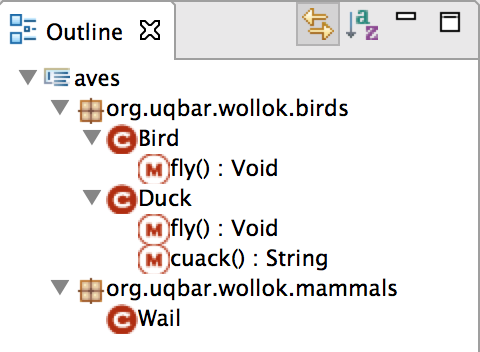
\includegraphics[scale=0.5]{images/wollok-paper-outline.png}
    \caption{Outline View: This view shows the structure of the file.}
    \label{fig:outline.png}
\end{figure}

% Interpreter
Wollok is implemented as a fully interpreted language, implemented as a Java application. 
The other standard XText implementation strategies involve generating Java code, which is very difficult to achieve out of a language without a single type annotation.
The downside of this decision is that we lost the \emph{out-of-the-box} type-checked code generation provided by XText, together with the XText standard debugger.

Regarding the debugger, we developed a custom eclipse plugin which already provides a good portion of the features provided by many industrial type language debuggers.
This debugger can even be abstracted into a reusable XText component for any other interpreted language.

% \subsection{Type System}
% XText type system is currently implemented on top of XSemantics\footnote{http://xsemantics.sourceforge.net}, a DSL for writing rules for XText languages. XSemantics is itself made with XText.
% This allows us to develop our type system in a declarative way. The type system can be seen in action in \figref{check-messageSending.png}.

\medskip
% \subsection{Development}
To allow for a graceful evolution of the language and the development environment, we also had to tailor our development practices.
While these ideas are not novel in indutrial developments, usually they do not have a lot of consideration in research projects or language development projects,
and a good bit of effort is required to adapt common industrial techniques to the specific needs of our project.

On one hand, we have been emphatic on the necessity for automated unit testing.
As said before, the difficulties which arise in testing a language implementation are quite challenging and different from other kinds of software.
Wollok combines several techniques for testing its development.
Part of the interpreter logic is being tested with unit tests in JUnit, 
while for the aspects that are more tied up with XText and Eclipse components we are using XPect\footnote{\url{http://www.xpect-tests.org}}, 
a unit and integration-testing framework for Xtext languages.
XPect is in turn also developed as an XText language.
It provides a declarative way to annotate Wollok programs with expected behaviour like validator’s errors/warnings, or code completions, etc.

On the othe hand, the deployment and distribution of Wollok is fully automated.
Combining several tools such as Github, Maven, Tycho, Travis CI, and Eclipse update sites we generated an infrastructure in which new versions can be released just with a pull request.
We have two distribution strategies: as a standalone product or as a plugin that can be added into any Eclipse instance.
Taking advantage of the Eclipse update sites, we allow the students to update their IDE without requiring a new installation.
This, in turn, allows us for a very fast development cycle for resolving potential errors or critical changes.
Finally, we distribute both \emph{stable} and \emph{development} versions. 
While the former are best for students, the latter are interesting for teachers which desire to get a glance of the new features in advance.
